\begin{tikzpicture}[
        font={\footnotesize},
        trap/.style={trapezium, rotate=-90,trapezium angle=75},
    ]
        %% CNN branch
        \node(input) at (0, 0) {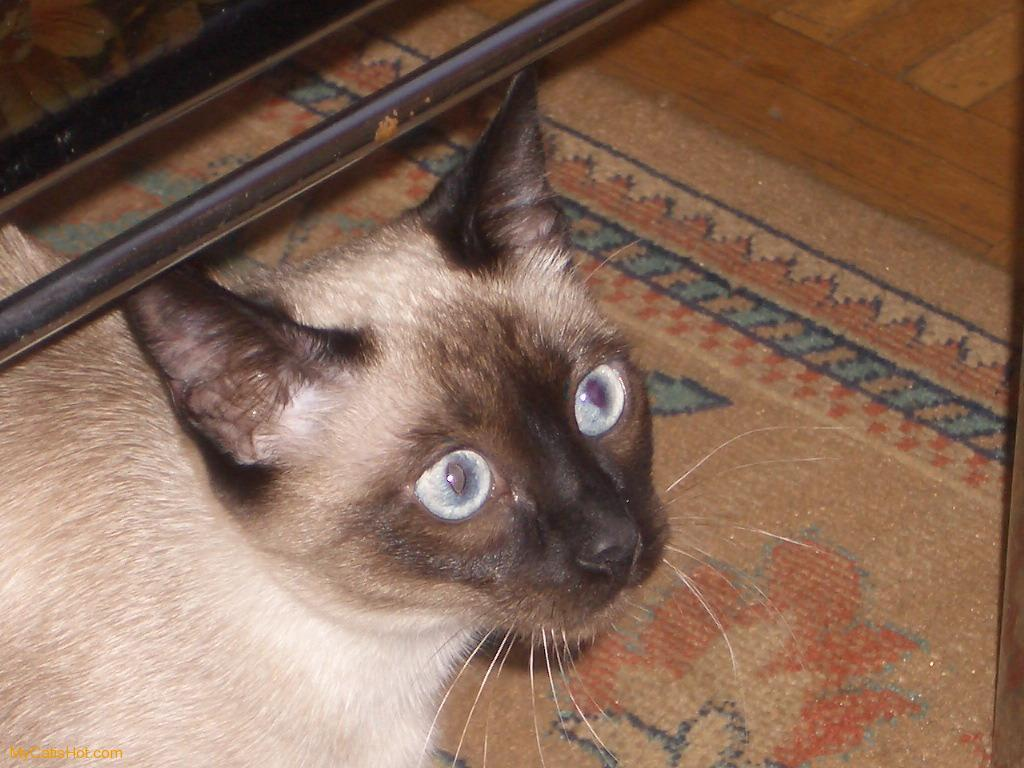
\includegraphics[width=.1\textwidth]{fig/castream/images/input.jpg}};
        \node[above] at (input.north) {Input image};
        \node[draw, rotate=90, align=center](conv1) at (2, 0) {\Th{conv} $7\times7$};
        %\node[draw, rotate=90, align=center](bn) at (-3, 0) {\Th{BatchNorm}};
        %\node[draw, rotate=90, align=center](relu) at (-2.5, 0) {\Th{ReLU}};
        %\node[draw, rotate=90, align=center](maxp) at (-2, 0) {\Th{MaxPool}};
        \node[draw, trap] (res1) at (4,0) {\rotatebox{90}{\parbox{1.0cm}{\centering{\Th{Res-1}}}}};
        \node[draw, trap] (res2) at (6,0) {\rotatebox{90}{\parbox{1.0cm}{\centering{\Th{Res-2}}}}};
        \node[draw, trap] (res3) at (8,0) {\rotatebox{90}{\parbox{1.0cm}{\centering{\Th{Res-3}}}}};
        \node[draw, trap] (res4) at (10,0) {\rotatebox{90}{\parbox{1.0cm}{\centering{\Th{Res-4}}}}};
        %\node[](empt1) at (6.25, 0){};
        \node[draw, rotate=90, align=center] (class) at (12,0) {Classifier};
        \node(logit) at (13, 0) {$\vy$};
    
        %% CNN backbone
        %\node(empt0) at (-4.65, 0) {};
        \draw[->] (input.east) -- node {} (conv1);
        \draw[->] (conv1.south) -- node[above] {$F_0$} (res1);
        %\draw[->] (empt0.center) -- node {} (conv1);
        \draw[->] (res1) -- node[above] {$F_1$} (res2);
        \draw[->] (res2) -- node[above] {$F_2$} (res3);
        \draw[->] (res3) -- node[above] {$F_3$} (res4);
        \draw[->] (res4) -- node [above] {} (class);
        \node[](GAP) at (11.125,0.25) {\gls{gap}};
        \draw[->] (class) -- node {} (logit);
\end{tikzpicture}
    